
\section{Design}

\subsection{System Architecture Diagrams}

\subsubsection{Component-Level Architecture}

The system integrates six hardware components around the Arduino Mega 2560 microcontroller. The keypad provides user input through a matrix GPIO interface, while the LCD receives status updates via I2C. The relay module is controlled by a single digital GPIO pin, and the PWM actuator (simulated by a blue LED) receives an analog-equivalent signal on a PWM-capable pin. Two status LEDs provide immediate visual feedback: green for normal operation and red for overload alert conditions.

\begin{figure}[H]
\centering
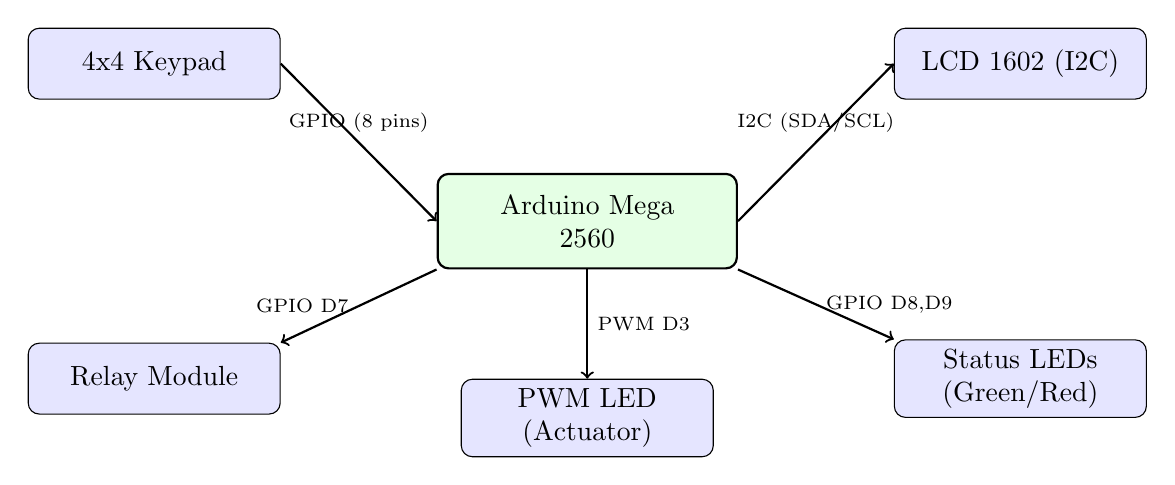
\begin{tikzpicture}[
    comp/.style={draw, rectangle, rounded corners, minimum width=3.2cm,
                 minimum height=0.9cm, text centered, align=center, fill=blue!10},
    mcu/.style={draw, rectangle, rounded corners, minimum width=3.8cm,
                minimum height=1.2cm, text centered, align=center, fill=green!10, thick}]
    \node[mcu]  (mega)   at (0,    0)    {Arduino Mega\\2560};
    \node[comp] (keypad) at (-5.5, 2.0)  {4x4 Keypad};
    \node[comp] (lcd)    at (5.5,  2.0)  {LCD 1602 (I2C)};
    \node[comp] (relay)  at (-5.5, -2.0) {Relay Module};
    \node[comp] (pwm)    at (0,    -2.5) {PWM LED\\(Actuator)};
    \node[comp] (leds)   at (5.5,  -2.0) {Status LEDs\\(Green/Red)};
    \draw[<-, thick] (mega.west) -- node[above, font=\scriptsize]{GPIO (8 pins)} (keypad.east);
    \draw[->, thick] (mega.east) -- node[above, font=\scriptsize]{I2C (SDA/SCL)} (lcd.west);
    \draw[->, thick] (mega.south west) -- node[left, font=\scriptsize]{GPIO D7} (relay.north east);
    \draw[->, thick] (mega.south) -- node[right, font=\scriptsize]{PWM D3} (pwm.north);
    \draw[->, thick] (mega.south east) -- node[right, font=\scriptsize]{GPIO D8,D9} (leds.north west);
\end{tikzpicture}
\caption{System structural diagram showing all hardware components and interfaces}
\label{fig:system_structural_diagram}
\end{figure}

\subsubsection{Layered System Architecture}

The software is organized into five layers following the AUTOSAR-inspired embedded systems architecture pattern. Each layer communicates only with its immediate neighbors, enforcing clean separation of concerns and enabling module reuse across labs.

\begin{figure}[H]
\centering
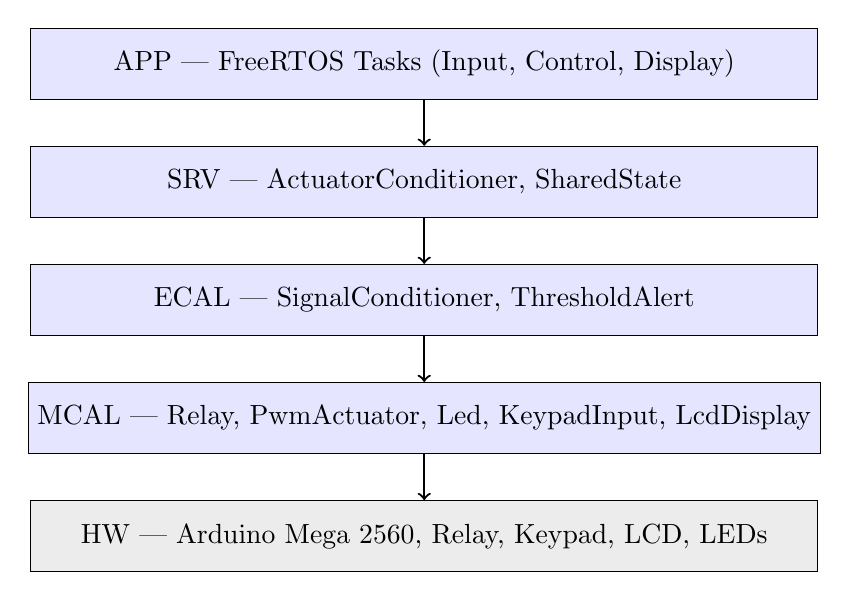
\begin{tikzpicture}[
    box/.style={draw, rectangle, minimum width=10cm, minimum height=0.9cm,
                text centered, fill=blue!10},
    node distance=0.4cm]
    \node[box] (app)  at (0, 0)    {APP --- FreeRTOS Tasks (Input, Control, Display)};
    \node[box] (srv)  at (0, -1.5) {SRV --- ActuatorConditioner, SharedState};
    \node[box] (ecal) at (0, -3.0) {ECAL --- SignalConditioner, ThresholdAlert};
    \node[box] (mcal) at (0, -4.5) {MCAL --- Relay, PwmActuator, Led, KeypadInput, LcdDisplay};
    \node[box, fill=gray!15] (hw) at (0, -6.0) {HW --- Arduino Mega 2560, Relay, Keypad, LCD, LEDs};
    \foreach \a/\b in {app/srv, srv/ecal, ecal/mcal, mcal/hw}
        \draw[->, thick] (\a) -- (\b);
\end{tikzpicture}
\caption{Layered software architecture of the dual-actuator control system}
\label{fig:layered_architecture}
\end{figure}

The APP layer contains the three FreeRTOS tasks and the lab entry point. The SRV layer provides the ActuatorConditioner (which wraps the SignalConditioner with ramping logic) and the SharedState module (mutex-protected data exchange). The ECAL layer implements the SignalConditioner pipeline and ThresholdAlert FSM as reusable, hardware-independent modules. The MCAL layer contains all hardware drivers that directly call Arduino GPIO, I2C, and PWM functions. The HW layer represents the physical components.

\subsection{Block Diagrams}

\subsubsection{Application Main Flowchart}

The application starts by initializing the serial interface, shared state, and spawning three FreeRTOS tasks. Once the scheduler starts, each task runs independently at its configured period.

\tikzset{
    startstop/.style={rectangle, rounded corners, minimum width=3cm,
        minimum height=0.7cm, text centered, align=center, draw=black, fill=gray!15},
    process/.style={rectangle, minimum width=3cm,
        minimum height=0.7cm, text centered, align=center, draw=black, fill=blue!10},
    arrow/.style={thick,->,>=Stealth}
}

\begin{figure}[H]
\centering
\begin{tikzpicture}
    \node (start)  [startstop] at (0,   0.0) {System Start};
    \node (serial) [process]   at (0,  -1.8) {Init STDIO Serial\\(9600 baud)};
    \node (shared) [process]   at (0,  -3.6) {Init SharedState\\+ Mutex};
    \node (tasks)  [process]   at (0,  -5.4) {Create 3 FreeRTOS\\Tasks};
    \node (sched)  [startstop] at (0,  -7.2) {Scheduler Runs\\(Tasks Active)};
    \draw [arrow] (start)  -- (serial);
    \draw [arrow] (serial) -- (shared);
    \draw [arrow] (shared) -- (tasks);
    \draw [arrow] (tasks)  -- (sched);
\end{tikzpicture}
\caption{Application initialization flowchart}
\label{fig:app_init_flowchart}
\end{figure}

\subsubsection{Input Task Flowchart}

The input task scans the keypad every 50\,ms and interprets the pressed key to update the shared actuator command state.

\begin{figure}[H]
\centering
\begin{tikzpicture}
    \tikzset{
        startstop/.style={rectangle, rounded corners, minimum width=2.8cm,
            minimum height=0.7cm, text centered, align=center, draw=black, fill=gray!15},
        process/.style={rectangle, minimum width=2.8cm,
            minimum height=0.7cm, text centered, align=center, draw=black, fill=blue!10},
        decision/.style={diamond, aspect=2.5, minimum width=2cm,
            minimum height=0.7cm, text centered, align=center, draw=black, fill=orange!15},
        arrow/.style={thick,->,>=Stealth}
    }
    \node (start)  [startstop] at (0,    0.0) {Wait 50\,ms};
    \node (scan)   [process]   at (0,   -1.8) {Scan Keypad};
    \node (dec1)   [decision]  at (0,   -4.3) {Key\\Pressed?};
    \node (lock)   [process]   at (0,   -6.8) {Lock Mutex};
    \node (proc)   [process]   at (0,   -8.6) {Process Key\\(A/B/C/D/0-9/\#/*)};
    \node (unlock) [process]   at (0,  -10.4) {Unlock Mutex};
    \draw [arrow] (start) -- (scan);
    \draw [arrow] (scan)  -- (dec1);
    \draw [arrow] (dec1)  -- node[anchor=east]{Yes} (lock);
    \draw [arrow] (dec1.east) -- ++(2.5, 0) node[above, font=\scriptsize]{No} |- (start.east);
    \draw [arrow] (lock)  -- (proc);
    \draw [arrow] (proc)  -- (unlock);
    \draw [arrow] (unlock.west) -- ++(-2.5, 0) |- (start.west);
\end{tikzpicture}
\caption{Input task flowchart --- keypad scanning and command interpretation}
\label{fig:input_task_flowchart}
\end{figure}

\subsubsection{Control Task Flowchart}

The control task runs every 100\,ms and applies debouncing to the relay command and the full conditioning pipeline to the PWM command.

\begin{figure}[H]
\centering
\begin{tikzpicture}
    \tikzset{
        startstop/.style={rectangle, rounded corners, minimum width=3cm,
            minimum height=0.7cm, text centered, align=center, draw=black, fill=gray!15},
        process/.style={rectangle, minimum width=3cm,
            minimum height=0.7cm, text centered, align=center, draw=black, fill=blue!10},
        arrow/.style={thick,->,>=Stealth}
    }
    \node (start)  [startstop] at (0,   0.0) {Wait 100\,ms};
    \node (lock)   [process]   at (0,  -1.8) {Lock Mutex\\Read Commands};
    \node (deb)    [process]   at (0,  -3.6) {Debounce Relay\\Command};
    \node (relay)  [process]   at (0,  -5.4) {Apply Relay\\State};
    \node (cond)   [process]   at (0,  -7.2) {Condition PWM\\(Sat$\to$Med$\to$EWMA$\to$Ramp)};
    \node (pwm)    [process]   at (0,  -9.0) {Apply PWM\\Output};
    \node (alert)  [process]   at (0, -10.8) {Evaluate Overload\\Alert FSM};
    \node (leds)   [process]   at (0, -12.6) {Update Status LEDs};
    \node (unlock) [process]   at (0, -14.4) {Unlock Mutex};
    \draw [arrow] (start)  -- (lock);
    \draw [arrow] (lock)   -- (deb);
    \draw [arrow] (deb)    -- (relay);
    \draw [arrow] (relay)  -- (cond);
    \draw [arrow] (cond)   -- (pwm);
    \draw [arrow] (pwm)    -- (alert);
    \draw [arrow] (alert)  -- (leds);
    \draw [arrow] (leds)   -- (unlock);
    \draw [arrow] (unlock.west) -- ++(-3.0, 0) |- (start.west);
\end{tikzpicture}
\caption{Control task flowchart --- actuator conditioning and hardware control}
\label{fig:control_task_flowchart}
\end{figure}

\subsubsection{Overload Alert FSM}

The overload detection uses a 4-state hysteresis FSM with debounce confirmation. An alert triggers when the conditioned PWM output exceeds 90\% for 3 consecutive evaluations, and clears when it drops below 80\% for 3 consecutive evaluations.

\begin{figure}[H]
\centering
\begin{tikzpicture}[>=Stealth, auto, node distance=3.5cm,
        every state/.style={draw, circle, minimum size=1.5cm, font=\scriptsize}]
    \node[state, initial]   (normal)  {NORMAL};
    \node[state]            (debH)    [right of=normal]  {DEB\_H};
    \node[state]            (alert)   [right of=debH]    {ALERT};
    \node[state]            (debL)    [below of=debH]    {DEB\_L};
    \path[->]
        (normal) edge              node[font=\tiny] {val $>$ 90\%}    (debH)
        (debH)   edge              node[font=\tiny] {3 confirms}      (alert)
        (debH)   edge [bend right] node[font=\tiny, below] {val $\leq$ 90\%} (normal)
        (alert)  edge              node[font=\tiny, right] {val $<$ 80\%}     (debL)
        (debL)   edge              node[font=\tiny] {3 confirms}      (normal)
        (debL)   edge [bend right] node[font=\tiny, right] {val $\geq$ 80\%} (alert);
\end{tikzpicture}
\caption{Overload alert FSM state diagram with hysteresis}
\label{fig:overload_fsm}
\end{figure}

\subsection{Electrical Schematics}

\subsubsection{Component Specification}

The circuit uses the following components with their electrical specifications:

\begin{itemize}
    \item \textbf{Arduino Mega 2560} --- MCU board, 5\,V logic, 16\,MHz, 54 digital I/O pins
    \item \textbf{Relay module} --- 5\,V single-channel, optocoupler-isolated, NO/NC/COM terminals
    \item \textbf{LCD 1602 I2C} --- 16x2 character display, I2C address 0x27, 5\,V supply
    \item \textbf{4x4 Keypad} --- membrane matrix, 8 GPIO lines (D22--D29)
    \item \textbf{Blue LED} --- PWM actuator indicator, $V_f \approx 3.0$\,V, with 220\,$\Omega$ resistor
    \item \textbf{Green LED} --- system normal indicator, $V_f \approx 2.1$\,V, with 220\,$\Omega$ resistor
    \item \textbf{Red LED} --- overload alert indicator, $V_f \approx 2.0$\,V, with 220\,$\Omega$ resistor
    \item \textbf{White LED} --- relay load indicator (connected through relay NO/COM)
\end{itemize}

\subsubsection{Circuit Connections}

The electrical schematic shows how each component connects to the Arduino Mega 2560. All LED circuits use 220\,$\Omega$ current-limiting resistors. The relay module receives its control signal from pin D7, while the PWM actuator LED is driven from pin D3. The keypad occupies pins D22--D29, and the LCD uses the I2C bus on pins D20 (SDA) and D21 (SCL).

\begin{figure}[H]
\centering
\begin{circuitikz}[scale=0.85, transform shape]
    % PWM LED circuit
    \draw (0,0) node[anchor=east]{\footnotesize Pin D3 (PWM)}
        to[R, l=220\,\si{\ohm}] (3,0)
        to[leD*, color=blue, l=\footnotesize PWM LED] (5.5,0)
        node[ground] {};

    % Green status LED
    \draw (0,-1.8) node[anchor=east]{\footnotesize Pin D8}
        to[R, l=220\,\si{\ohm}] (3,-1.8)
        to[leD*, color=green, l=\footnotesize Green] (5.5,-1.8)
        node[ground] {};

    % Red alert LED
    \draw (0,-3.6) node[anchor=east]{\footnotesize Pin D9}
        to[R, l=220\,\si{\ohm}] (3,-3.6)
        to[leD*, color=red, l=\footnotesize Red] (5.5,-3.6)
        node[ground] {};

    % Relay control
    \draw (0,-5.4) node[anchor=east]{\footnotesize Pin D7}
        to[short] (2,-5.4)
        node[anchor=west]{\footnotesize Relay IN};

    % Relay load circuit
    \draw (4,-5.4) node[anchor=east]{\footnotesize Relay COM}
        to[leD*, color=white, l=\footnotesize Load LED] (7,-5.4)
        node[ground] {};
    \draw (4,-6.4) node[anchor=east]{\footnotesize Relay NC}
        to[short] (5,-6.4)
        node[anchor=west]{\footnotesize 5V};

    % I2C LCD
    \draw (0,-8.0) node[anchor=east]{\footnotesize Pin D20 (SDA)}
        to[short] (3,-8.0) node[anchor=west]{\footnotesize LCD SDA};
    \draw (0,-9.0) node[anchor=east]{\footnotesize Pin D21 (SCL)}
        to[short] (3,-9.0) node[anchor=west]{\footnotesize LCD SCL};
\end{circuitikz}
\caption{Circuit schematic of the dual-actuator control system}
\label{fig:circuit_schematic}
\end{figure}

\subsubsection{Hardware Configuration}

The Wokwi simulation configuration uses a breadboard to route connections between the Arduino Mega and peripheral components. The keypad, LEDs with resistors, and power/ground rails all pass through the breadboard, closely resembling a physical prototyping setup.

\begin{lstlisting}[language=json, caption=Wokwi configuration file (wokwi.toml), label=lst:wokwi_config]
[wokwi]
version = 1
firmware = "../../.pio/build/lab4/firmware.hex"
elf = "../../.pio/build/lab4/firmware.elf"
\end{lstlisting}

\begin{figure}[H]
\centering
\IfFileExists{resources/Design/ElectricalSchematics/wokwi_circuit.png}{%
    
\includegraphics[width=0.85\textwidth]{resources/Design/ElectricalSchematics/wokwi_circuit.png}%
}{%
    \fbox{\parbox{0.83\textwidth}{\centering\color{gray}\small
        [Screenshot pending --- run the Wokwi simulation and save to\\
        resources/Design/ElectricalSchematics/wokwi\_circuit.png]}}%
}
\caption{Wokwi simulation circuit with breadboard layout (active run)}
\label{fig:wokwi_circuit}
\end{figure}

\subsection{Project Structure}

\begin{lstlisting}[caption=Project directory structure for Lab 4, label=lst:project_structure]
labs/
|-- platformio.ini
|-- src/
|   |-- main.cpp              (lab selector entry point)
|-- lab/
|   |-- lab4/
|       |-- lab4_main.cpp/h   (lab entry point)
|       |-- lab4_config.h     (pin mapping + config)
|       |-- shared_state.cpp/h (mutex-protected shared data)
|       |-- task_input.cpp/h  (keypad scanning task)
|       |-- task_control.cpp/h (actuator control task)
|       |-- task_display.cpp/h (LCD + serial reporting task)
|-- lib/
|   |-- Relay/                (binary actuator driver)
|   |-- PwmActuator/          (analog actuator driver)
|   |-- ActuatorConditioner/  (command conditioning + ramp)
|   |-- SignalConditioner/    (saturate/median/EWMA pipeline)
|   |-- ThresholdAlert/       (hysteresis alert FSM)
|   |-- KeypadInput/          (4x4 keypad driver)
|   |-- LcdDisplay/           (I2C LCD driver)
|   |-- Led/                  (LED driver)
|   |-- StdioSerial/          (STDIO serial redirect)
|-- wokwi/
    |-- lab4/
        |-- diagram.json
        |-- wokwi.toml
\end{lstlisting}

\subsection{Modular Implementation}

\subsubsection{MCAL Layer: Relay Driver}

The Relay module provides a simple interface for controlling a relay connected to a digital GPIO pin. It supports configurable active level (HIGH or LOW) and tracks the current relay state internally.

\begin{lstlisting}[language=C++, caption=Relay driver interface (Relay.h), label=lst:relay_h]
class Relay {
public:
    Relay(uint8_t pin, bool activeHigh = true);
    void init();
    void turnOn();
    void turnOff();
    void toggle();
    void setState(bool on);
    bool isOn() const;
private:
    uint8_t _pin;
    bool    _activeHigh;
    bool    _state;
};
\end{lstlisting}

The implementation maps the logical ON/OFF state to the physical pin level based on the \texttt{activeHigh} configuration. When \texttt{activeHigh} is true, turning ON writes HIGH to the pin; when false, it writes LOW. This accommodates both active-HIGH relay modules (common in Arduino ecosystem) and active-LOW modules (common in industrial applications).

\subsubsection{MCAL Layer: PWM Actuator Driver}

The PwmActuator module abstracts PWM output control, accepting a duty cycle percentage (0--100\%) and mapping it to the 8-bit range required by \texttt{analogWrite()}.

\begin{lstlisting}[language=C++, caption=PwmActuator driver interface (PwmActuator.h), label=lst:pwm_actuator_h]
class PwmActuator {
public:
    PwmActuator(uint8_t pin);
    void init();
    void setDuty(float duty);
    float getDuty() const;
    uint8_t getRawPwm() const;
private:
    uint8_t _pin;
    float   _duty;
};
\end{lstlisting}

The \texttt{setDuty()} method clamps the input to [0, 100] before computing \texttt{pwmVal = duty * 255 / 100} and calling \texttt{analogWrite()}. This percentage-based interface decouples the application logic from the hardware-specific 8-bit range.

\subsubsection{SRV Layer: Actuator Conditioner}

The ActuatorConditioner module extends the existing SignalConditioner with a ramping stage. It wraps the three-stage pipeline (saturation, median filter, EWMA) and adds gradual output transitions to protect mechanical actuators from sudden changes.

\begin{lstlisting}[language=C++, caption=ActuatorConditioner interface (ActuatorConditioner.h), label=lst:act_cond_h]
class ActuatorConditioner {
public:
    ActuatorConditioner(uint8_t medianWindow, float ewmaAlpha,
                        float minClamp, float maxClamp,
                        float maxRampStep);
    float process(float rawCommand);
    float getRampedOutput() const;
    float getConditionedTarget() const;
    const SignalConditioner& getSignalConditioner() const;
    void reset();
};
\end{lstlisting}

The ramping logic computes the difference between the conditioned target and the current output, then limits the change to \texttt{maxRampStep} per call. This ensures that even if the user commands a jump from 0\% to 100\%, the actual output ramps up at 5\% per 100\,ms cycle, reaching full speed in approximately 2 seconds.

\subsubsection{APP Layer: Shared State Module}

The SharedState module defines the \texttt{ActuatorState} structure containing all data exchanged between the three tasks: relay command/actual state, PWM command/conditioned/ramped values, alert status, and input mode tracking. A FreeRTOS mutex protects concurrent access.

\begin{lstlisting}[language=C++, caption=Shared state structure (shared\_state.h), label=lst:shared_state_h]
struct ActuatorState {
    bool relayCommandOn;
    bool relayActualOn;
    uint8_t relayDebounceCount;
    float pwmCommandPercent;
    float pwmConditioned;
    float pwmRamped;
    uint8_t pwmRawValue;
    bool overloadAlert;
    bool inputModeAnalog;
    char inputBuffer[4];
    uint8_t inputBufferLen;
};
\end{lstlisting}

\subsubsection{APP Layer: FreeRTOS Tasks}

Three tasks run concurrently, each with a dedicated period and priority. The Input task (priority 3, 50\,ms) has the highest priority to ensure responsive keypad scanning. The Control task (priority 2, 100\,ms) processes actuator commands and drives hardware. The Display task (priority 1, 500\,ms) updates the LCD and prints serial reports at a relaxed rate to avoid consuming excessive CPU time with I/O operations.

All tasks follow the same pattern: acquire the mutex, read/write the shared state, release the mutex, then perform hardware I/O outside the critical section where possible. This minimizes mutex hold time and reduces the risk of priority inversion.
